\section{Deep Learning}
\label{sec:deeplearning}

In \refsec{neural}, we introduced neural networks with hidden layers and the backpropagation algorithm to fit them,
both of which date back to at least the 1970's.
In the past decade, however, the Artificial Intelligence community is transformed by the introduction of \concept{deep learning},
where deep refers to a large amount of hidden layers between the input and output layers.
Many of the recent advances in AI, from self-driving cars to automatic translation and voice assistants,
are made possible by the application of deep learning techniques to the enormous amounts of digital data now becoming available. 

An extensive treatment of Deep Learning is beyond the scope of this book (we recommend \cite{geron2019hands} instead).
However, in this section we will give you a brief introduction that should help you understand deep learning at a conceptual level,
and in \refchap{dtm} and \refchap{image} we will explain how these techniques can be applied to text analysis and visual analysis, respectively. 

In principle, there is no clear demarcation between a `classical' neural network with hidden layers and a `deep' neural network.
There are three properties, however, that distinguish deep learning and explain why it is so succesful: scale, structure, and feature learning.

\paragraph{Scale} First, and perhaps most importantly, deep learning models are many orders of magnitude larger and more complex than the models
trained in earlier decades.
This has been made possible by the confluence of unprecedented amounts of digital training data and increased computer processing power.
Party, this is enabled by the use of graphical processing units (GPUs), hardware designed for rendering the 3D worlds used in games,
but that can also be used very efficiently for the computations needed to train neural networks (and mine bitcoins, but that's another story).

\paragraph{Structure} Most classical neural networks have only `fully connected' hidden layers with forward propagation,
meaning that each neuron in one layer is connected to each neuron in the next layer.
In deep learning, many specific architectures (some of which will be discussed below) are used to process information in certain ways,
limiting the number of parameters that need to be estimated.

\paragraph{Feature Learning}
In all models described so far with the exception of neural networks with hidden layers,
there was a direct relationship between the input features and the output class.
This meant that it is important to make sure that the required information the model needs to distinguish the classes
is directly encoded in the input features.
In the example used earlier, if `not' and `good' are separate features, a single-layer network (or a naive bayes model)
cannot learn that these words together have a different meaning than the addition of their separate meanings.
However, similar to regression analysis, where you can create an interaction term or squared term to model a non-linear relationship,
the researcher can create input features for e.g. word pairs, for example including bigrams (word pars) such as `not\_good`.
In fact, engineering the right features was the main way in which a researcher could improve model performance.
In deep learning, however, this feature learning step is generally included in the model itself,
with subsequent layers encoding different aspects of the raw data.

The properties of scale, structure, and feature learning are intertwined in deep learning: the much larger networks enable structures with beautiful names such as `recurrent networks,' `convolutional layers' or `long short-term memory',
which are used to encode specific relationships and dependencies between features.
In this book, we will focus on convolutional networks as our only example of deep learning,
mostly because these networks are widely used in both text and image analysis.
Hopefully, this will give you insight into the general idea behind deep learning,
and you can learn about this and other models in more detail in the specialized resources cited above.  

\subsection{Convolutional Neural Networks}
\label{sec:cnnbasis}

One challenge in many machine learning problems is a mismatch between the level of measurement of the output and the input.
For example, we normally want to  assign a single code such as sentiment or topic to a document or image.
The raw input, however, is at the word or pixel level.
In classical machine learning, this is generally solved by summarizing the input at the higher level of abstraction,
for example by using the total frequency of each word per document as input feature.
The problem is, however, that this summarization process removes a lot information that could be useful to the machine learning model,
for example combinations of words (`not good') or their ordering (`John voted for Mary' vs `Mary voted for John'),
unless the researcher engineers features such as word pairs to add this information.

Convolutional Neural Networks are one way in which deep learning can overcome this limitation.
Essentially, the model internalizes the feature learning as a first part or `layer' of the model,
using a specialized network to summarize the raw input values into document (or image) lewvel features. 

\begin{figure}
  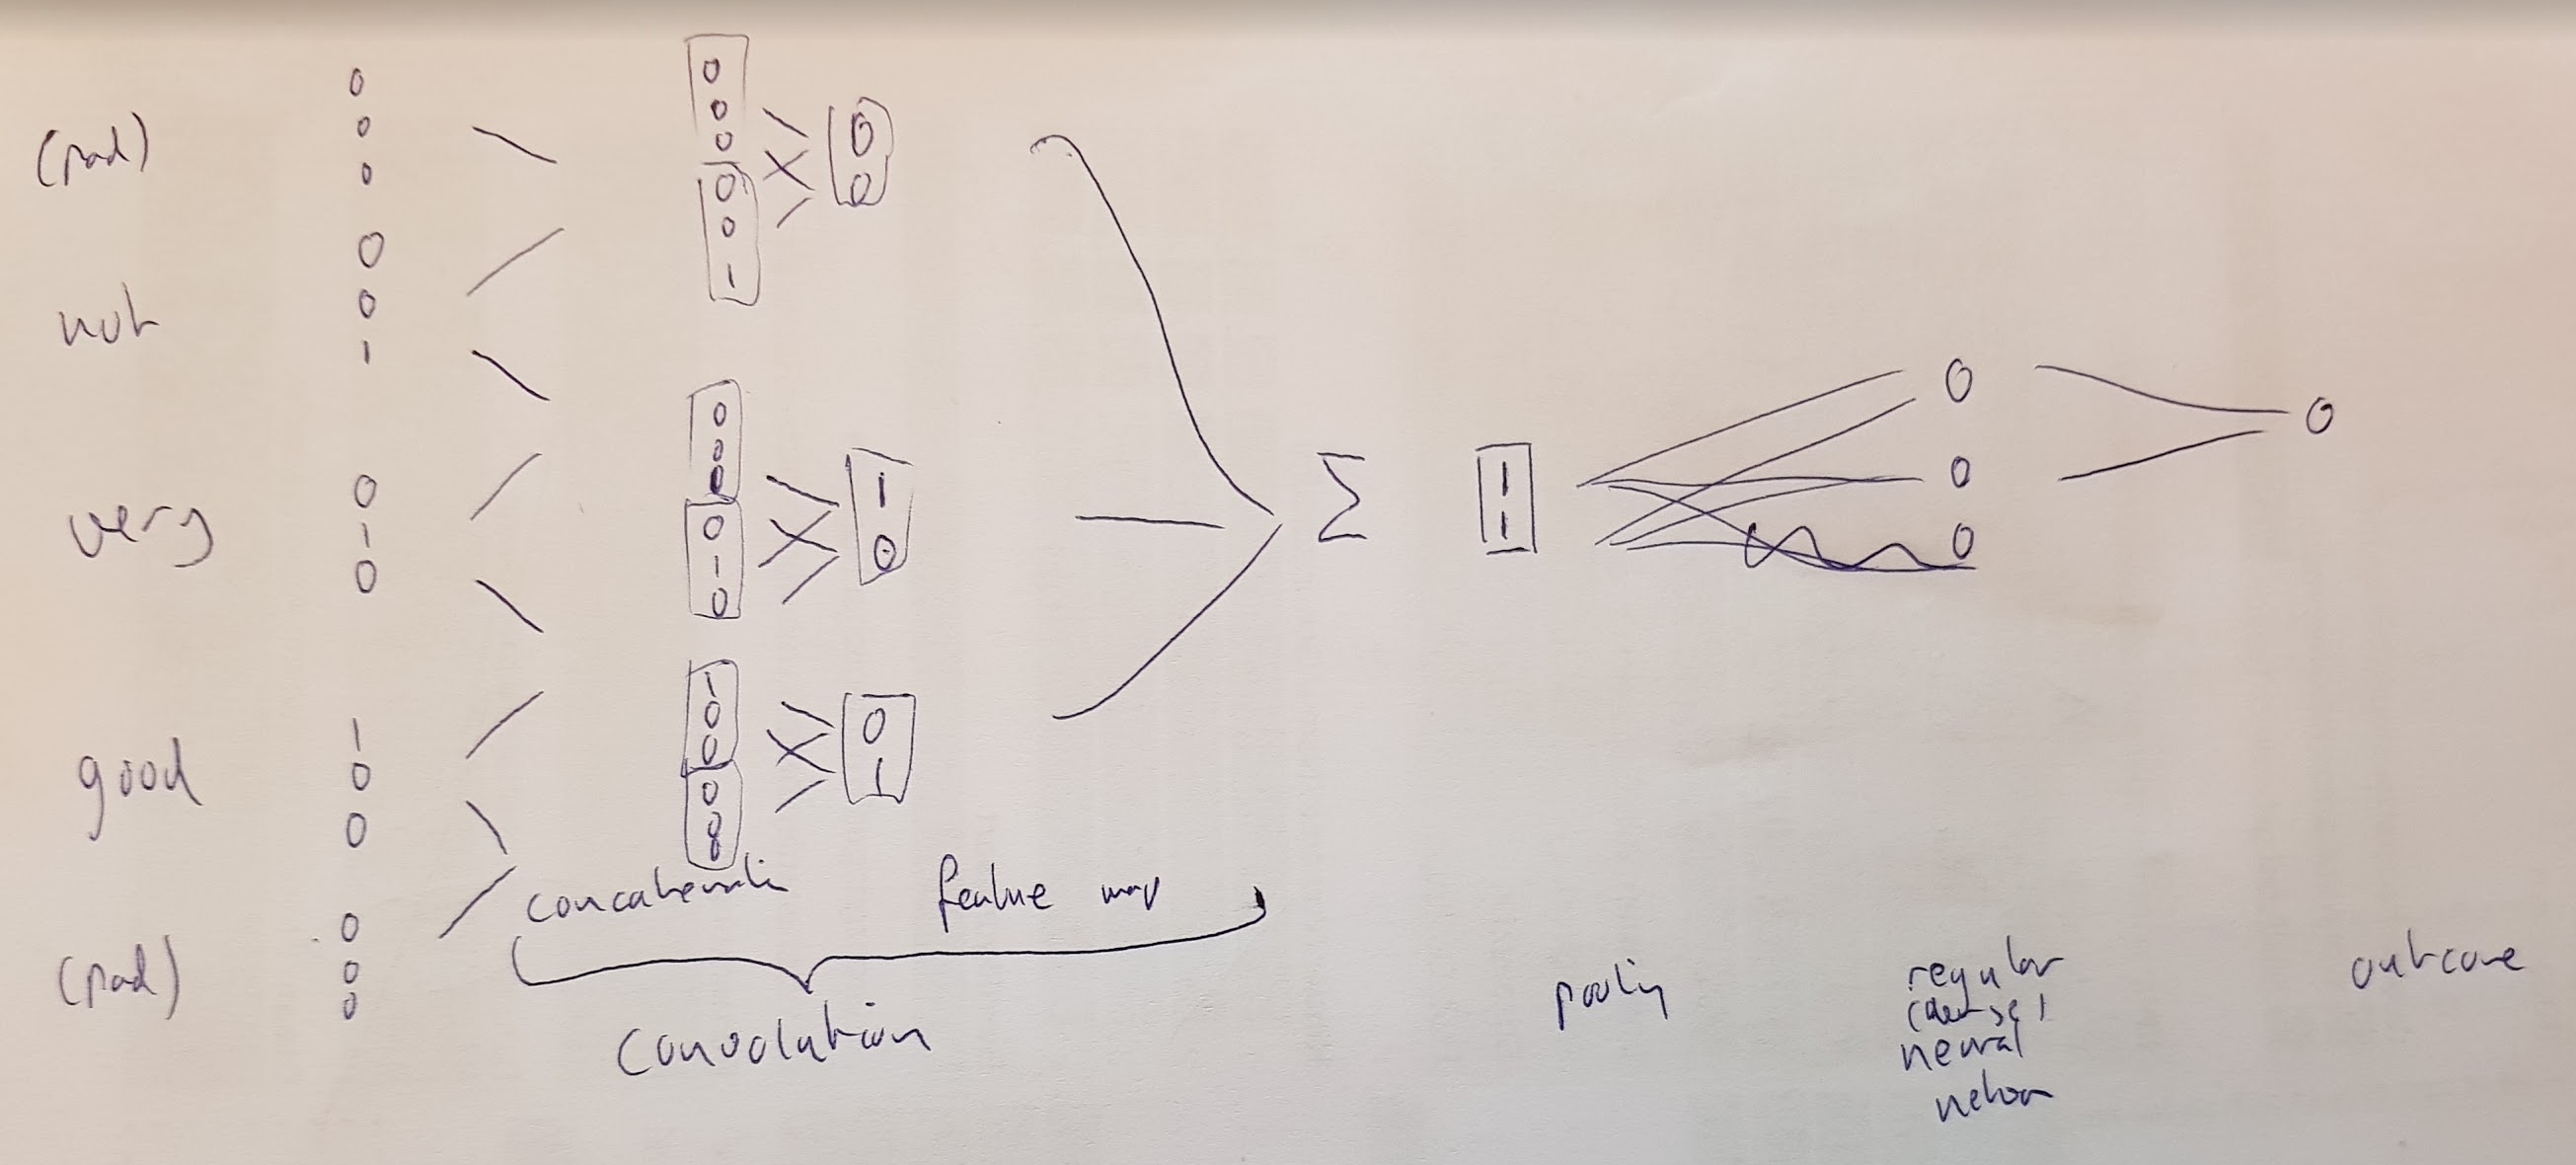
\includegraphics[width=\linewidth]{figures/ch09_cnn.png}
  \caption{Simplified example of a Convolutional Network applied to text analysis}
  \label{fig:cnn}
  \end{figure}

\reffig{cnn} shows a highly simplified example of this for text analysis of a sentence fragment `Would not recommend'.
The left hand shows how each word is encoded as a binary vector (e.g. 010 for `not', and 001 for `recommend').
In the second column, a shifting window concatenates these values for word pairs (so 010001 for `not recommend').
Next, a feature map layer detects interesting features in these concatenated values, for example
a feature for a negated positive term that has positive weights for negators in the first half and for positive words in the second.
These features are then pooled together to create document-level features,
for example by taking the maximum value per feature, which means that a feature is present in a document if it is present in any of the word windows in the document.
Finally, these document-level features are then used in a regular (dense) neural network which is connected to the output value, e.g. the document sentiment.
Since the convolutional layer is now connected with the output class, the feature maps can be automatically learned using the backpropagation algorithm explained above.
This means that the model can find the features in the word windows that are most helpful in predicting the document class, bringing the feature learning into the modelling process.

Of course, this is a highly simplified example, but it shows how local dependencies can be detected automatically using the convolutional network, as long as the interesting features are found within the specified word window.
Other architectures, such as the Long Short Term Memory mentioned above, can be used to also find non-local dependencies, but a full discussion of different architectures is well beyond the scope of this book. 
\refchap{dtm} will give a more detailed example of deep learning for text analysis, where an embedding layer is combined with a convolutional network to build a sentiment analysis model.
Similarly, \refchap{image} will show how a similar technique can be used to extract features from small areas of images which are then used in automatic image classification.
This involves creating a two dimensional window over pixels rather than a unidimensional window over words, and often multiple convolutional layers are chained to detect features in increasingly large areas of the image.
The underlying technique of convolutional netoworks, however, is the same in both cases.
